\chapter{Data and Model Exploration} %%%%%%%%%%%%%%%%%%%%%%%%%%%%%%%%%%%%%%%%%%%%%%%%%%%%%%%%
\label{chap:data_exploration}

With the increasing adoption of machine learning across all industries, the data used for training a DNN model has become a key component for its success. It is essential that for supervised machine learning, the training data is classified into various categories. For example, if there are 2 classes of images for the machine learning model to recognise, say a cat and dog, these images must be labeled containing these two classes of animals.

In this chapter, the dataset used for the thesis is discussed using various visualization techniques. Seed models developed for classifying the dataset are also discussed in the later sections.

\section{Dataset}

The data used for the experiments is a two-channel anonymous ECG dataset. The ECG data is in a mixed text/binary format with the data stored as a 16-bit little-endian integer. The data is already collected and it is stored in ".ecg" files. Since it is the ECG data, we have voltage values stored in the file. 

\section{Data description}
\label{sec:data_description}
The voltage value of the ECG signal is the amplitude with respect to a value over a period of 120-180 seconds. To retrieve the voltage value from the 16-bit values from the stream of data in the ".ecg" file, we subtract value of the "offset" from the actual values and then multiply the result by "factor". The "offset" and "factor" are header values which are obtained from each ".ecg" file and are constant values for that particular ECG signal. This is used to normalize the data in our case. The formula, as such, to calculate the value (or the amplitude of the signal) is:

\[ (value\hspace{1mm} -\hspace{1mm} offset)\hspace{1mm} \mbox{*}\hspace{1mm} factor = amplitude\hspace{2mm} in\hspace{2mm} millivolts\hspace{2mm}(\textbf{mV}) \]

For an example, if the 16-bit binary value after decoding (with little endian format) is 2287, if "offset" from the header is 2048 and "factor" is 0.002930, then the amplitude is :

\[ (2287 - 2048)\hspace{1mm} \mbox{*}\hspace{1mm} 0.002930 = 0.70027\hspace{2mm} mV \]

An example for the header in the ".ecg" files is shown below in table ~\ref{tab:ecg_header_example}:

\begin{table}[ht]
    \begin{tabular}{ll}
    \hline
        \multicolumn{2}{c}{Example for the text header} \\
    \hline
    Type:                  & CL1000\_ECG               \\
    Sample rate:           & 1024.000000               \\
    Offset:                & 0.000000                  \\
    Unit:                  & mV                        \\
    Factor:                & - 0.002441                \\
    Compression:           & 0                         \\
    Device:                & CL3000                    \\
    Device SN:             & 041 04 0072               \\
    DateOfLastCalibration: & 06/17/2003 12: 46: 11,000 \\
    PortName:              & USB                       \\
    Driver name:           & d\_comm.dll               \\
    Driver version:        & 1.1.0.9                   \\
    Time of first sample:  & 0                         \\
    Channels:              & 8th                       \\
    Channel Names:         & I II V1 V2 V3 V4 V5 V6    \\
    \hline
    \end{tabular}
    \caption{Example for ECG header in the "*.ecg" files }
    \label{tab:ecg_header_example}
\end{table}

The sampling frequency (or sample rate) is also part of the header of the ".ecg" file. This is used to calculate the duration of the signal. The data stream consists of data from \textbf{2 channels} for this duration. If the USB device used to collect the data was temporarily disconnected during the recording or if the transmission was disturbed, then this period in the signal will contain zero values. If there are gaps in the ECG, then these gaps are also filled with zero values. These zero values must also be accounted for when decoding the data. It is also noted that binary data is aligned on 8-byte boundaries and sometimes, the data must be moved to the beginning of this 8-byte aligned data manually when reading the ".ecg" file.

\clearpage
\section{Data Visualization}
\label{sec:data_visulization}
ECG signals can have different waveforms and morphologies. Similar to many other time-series data, the main problem with the manual analysis of ECG signals lies in the difficulty of detecting and categorizing these different waveforms and morphologies into the various classes. The current dataset of the ECG consists of 2 classes of data. The two classes are sinus rhythm and atrial fibrillation rhythm. Atrial fibrillation is the irregular heartbeat, or arrhythmia, whereas the sinus rhythm is the regular heartbeat.

The dataset consists of 8,000 files for sinus rhythm and 8,000 files for atrial fibrillation. The dataset, as per the usual conventions, is divided into 70\% for training, 15\% for validation and 15\% for testing. This results in:
\begin{itemize}
    \item 5,600 files for training - for sinus
    \item 5,600 files for training - for atrial fibrillation
    \item 1200 files for validation - for sinus
    \item 1200 files for validation - for atrial fibrillation
    \item 1200 files for testing - for sinus
    \item 1200 files for testing - for atrial fibrillation
\end{itemize}

Visualization for few of the ".ecg " files are provided in following figures.

\begin{figure}[ht!]
\centering
    \begin{minipage}{.5\textwidth}
      \centering
        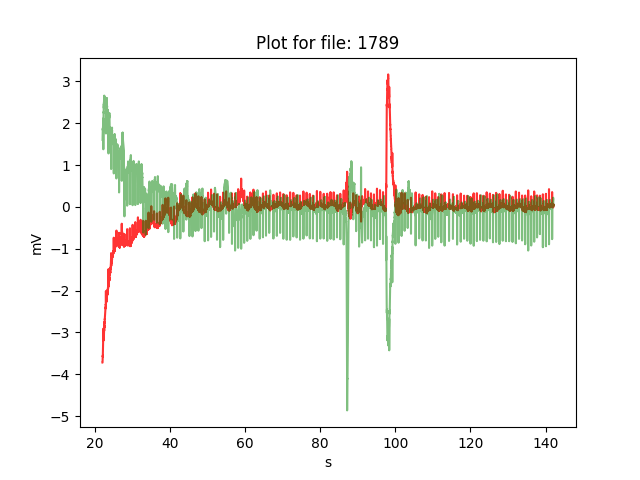
\includegraphics[width=1.0\linewidth, height=5cm]{BachelorMasterThesis/DataExploration/Figures/sinus/ecg/1789.png}
            % \captionof{figure}{Mathematical model of the neuron 3}
            \label{fig:sinus_1}
        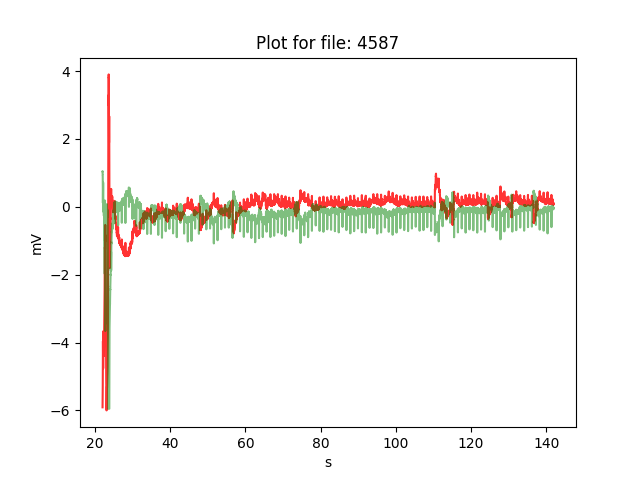
\includegraphics[width=1.0\linewidth, height=5cm]{BachelorMasterThesis/DataExploration/Figures/sinus/ecg/4587.png}
            % \captionof{figure}{Mathematical model of the neuron 2}
            \label{fig:sinus_2}
        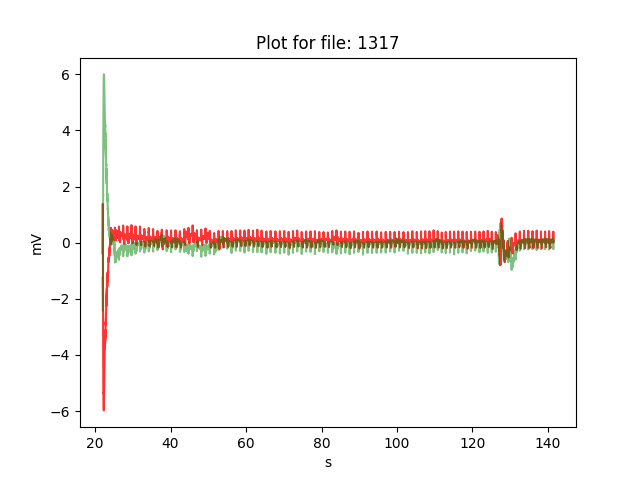
\includegraphics[width=1.0\linewidth, height=5cm]{BachelorMasterThesis/DataExploration/Figures/sinus/ecg/1317.png}
            % \captionof{figure}{Biological Neuron 1}
            \label{fig:sinus_3}
        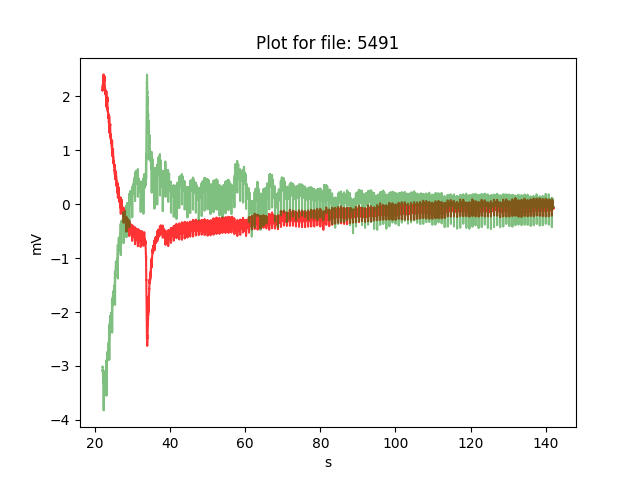
\includegraphics[width=1.0\linewidth, height=5cm]{BachelorMasterThesis/DataExploration/Figures/sinus/ecg/5491.png}
            % \captionof{figure}{Mathematical model of the neuron 4}
            \label{fig:sinus_4}
    \end{minipage}%
    \begin{minipage}{.5\textwidth}
      \centering
        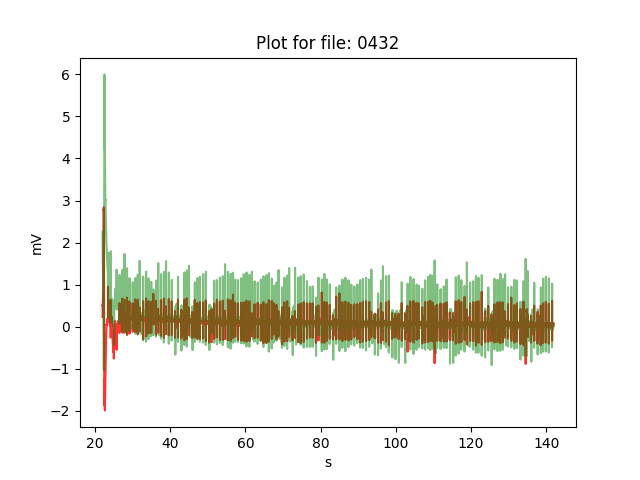
\includegraphics[width=1.0\linewidth, height=5cm]{BachelorMasterThesis/DataExploration/Figures/atrial_fibrillation/ecg/0432.png}
            % \captionof{figure}{Biological Neuron 1}
            \label{fig:af_1}
        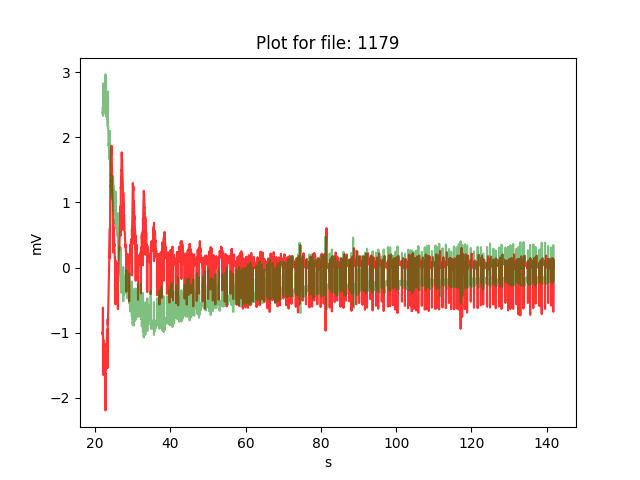
\includegraphics[width=1.0\linewidth, height=5cm]{BachelorMasterThesis/DataExploration/Figures/atrial_fibrillation/ecg/1179.png}
            % \captionof{figure}{Mathematical model of the neuron 3}
            \label{fig:af_2}
        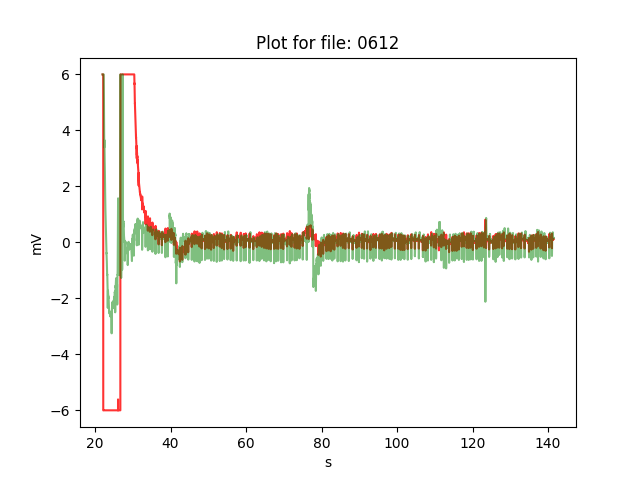
\includegraphics[width=1.0\linewidth, height=5cm]{BachelorMasterThesis/DataExploration/Figures/atrial_fibrillation/ecg/0612.png}
            % \captionof{figure}{Mathematical model of the neuron 2}
            \label{fig:af_3}
        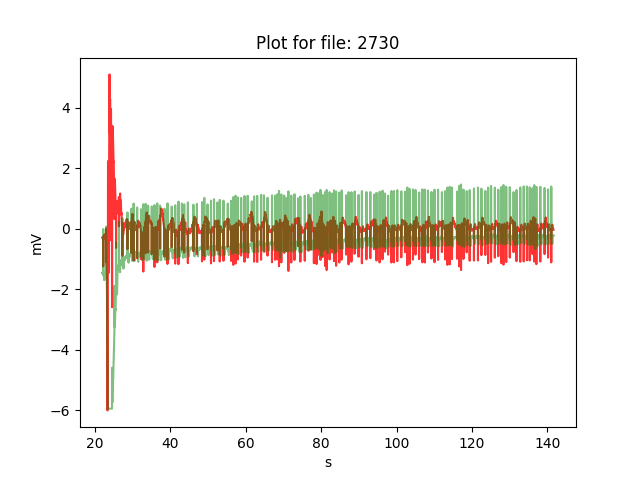
\includegraphics[width=1.0\linewidth, height=5cm]{BachelorMasterThesis/DataExploration/Figures/atrial_fibrillation/ecg/2730.png}
            % \captionof{figure}{Mathematical model of the neuron 4}
            \label{fig:af_4}
    \end{minipage}
    \caption{ECG signal of Sinus (left) vs Atrial fibrillation (right)}
    \label{fig:ecg_sinus_vs_af}
\end{figure}

\begin{figure}[ht!]
\centering
    \begin{minipage}{.5\textwidth}
      \centering
        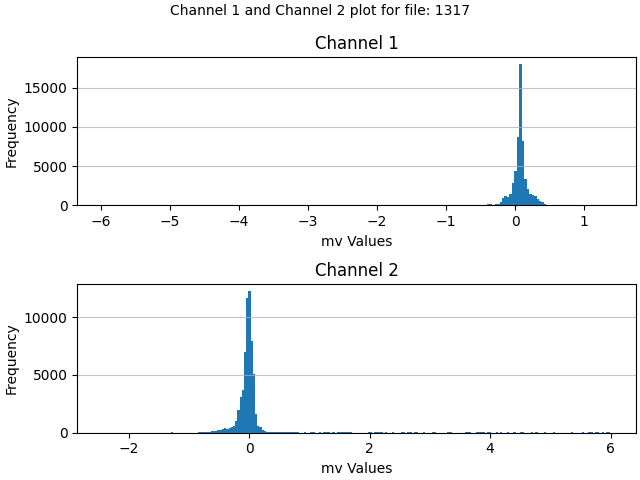
\includegraphics[width=1.0\linewidth, height=8cm]{BachelorMasterThesis/DataExploration/Figures/sinus/histogram/1317.png}
            % \captionof{figure}{Mathematical model of the neuron 3}
            \label{fig:sinus_histogram_1}
        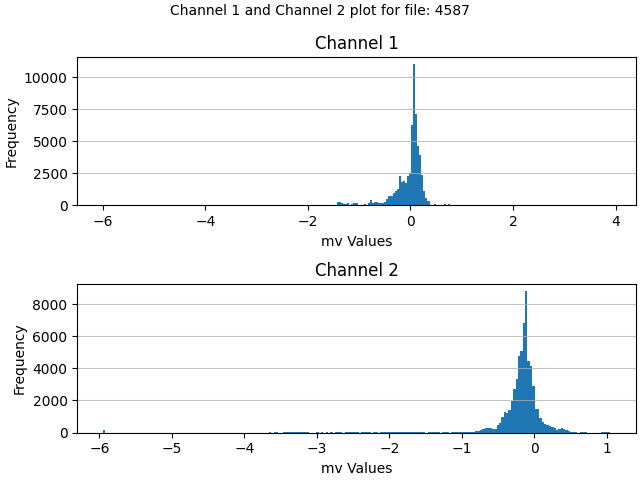
\includegraphics[width=1.0\linewidth, height=8cm]{BachelorMasterThesis/DataExploration/Figures/sinus/histogram/4587.png}
            % \captionof{figure}{Mathematical model of the neuron 2}
            \label{fig:sinus_histogram_2}
    \end{minipage}%
    \begin{minipage}{.5\textwidth}
      \centering
        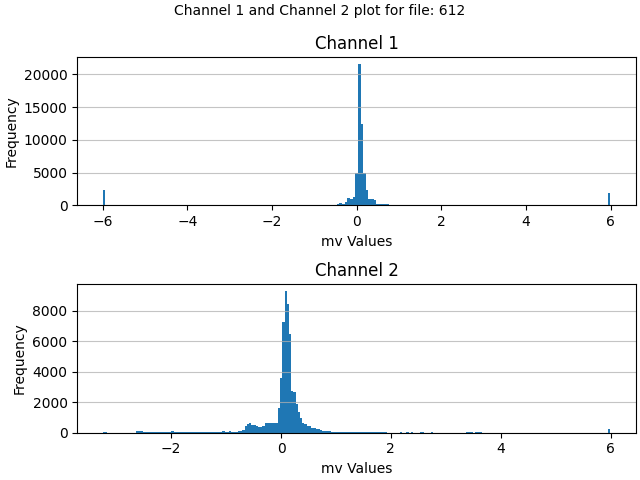
\includegraphics[width=1.0\linewidth, height=8cm]{BachelorMasterThesis/DataExploration/Figures/atrial_fibrillation/histogram/612.png}
            % \captionof{figure}{Biological Neuron 1}
            \label{fig:af_histogram_1}
        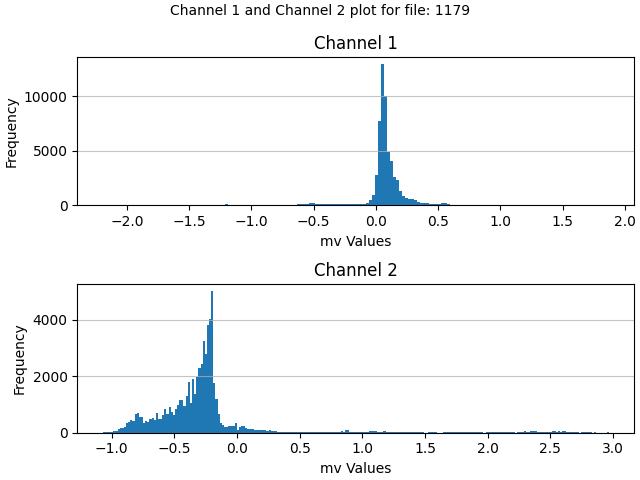
\includegraphics[width=1.0\linewidth, height=8cm]{BachelorMasterThesis/DataExploration/Figures/atrial_fibrillation/histogram/1179.png}
            % \captionof{figure}{Mathematical model of the neuron 3}
            \label{fig:af_histogram_2}
    \end{minipage}
    \caption{ECG signal distribution - Histogram - of Sinus (left) vs Atrial fibrillation (right)}
    \label{fig:ecg_histogram_plot_1_sinus_vs_af}
\end{figure}

% \begin{figure}[ht!]
% \centering
%     \begin{minipage}{.5\textwidth}
%       \centering
%         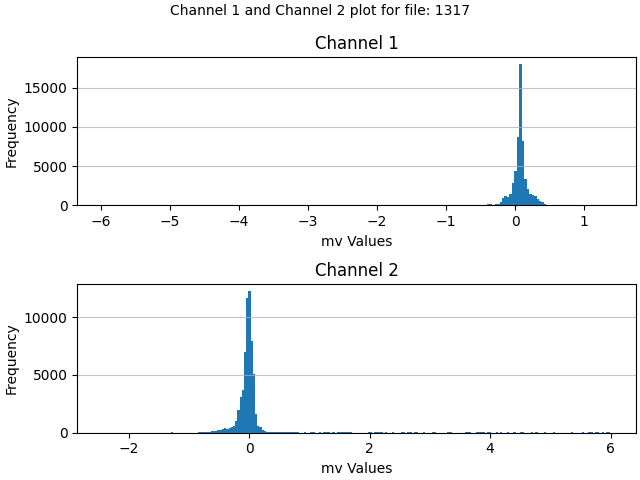
\includegraphics[width=1.0\linewidth, height=8cm]{BachelorMasterThesis/DataExploration/Figures/sinus/histogram/1317.png}
%             % \captionof{figure}{Biological Neuron 1}
%             \label{fig:sinus_histogram_3}
%         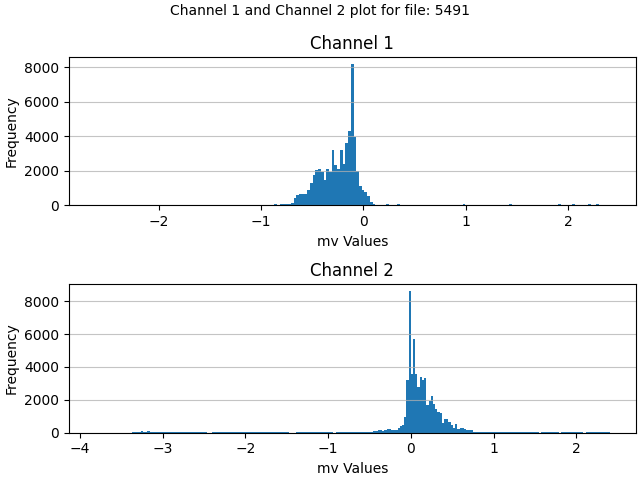
\includegraphics[width=1.0\linewidth, height=8cm]{BachelorMasterThesis/DataExploration/Figures/sinus/histogram/5491.png}
%             % \captionof{figure}{Mathematical model of the neuron 4}
%             \label{fig:sinus_histogram_4}
%     \end{minipage}%
%     \begin{minipage}{.5\textwidth}
%       \centering
%         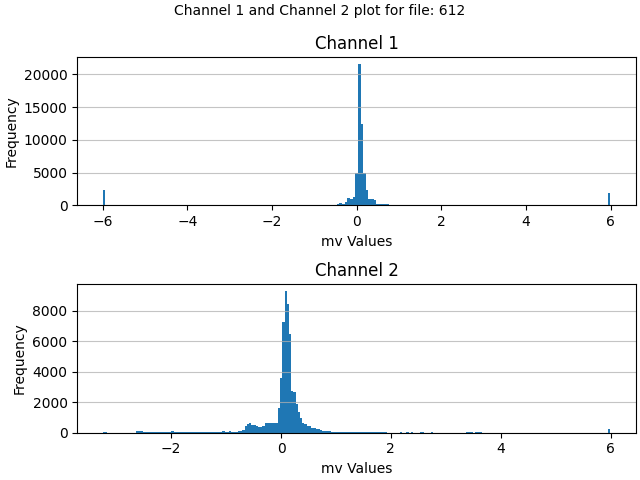
\includegraphics[width=1.0\linewidth, height=8cm]{BachelorMasterThesis/DataExploration/Figures/atrial_fibrillation/histogram/612.png}
%             % \captionof{figure}{Mathematical model of the neuron 2}
%             \label{fig:af_histogram_3}
%         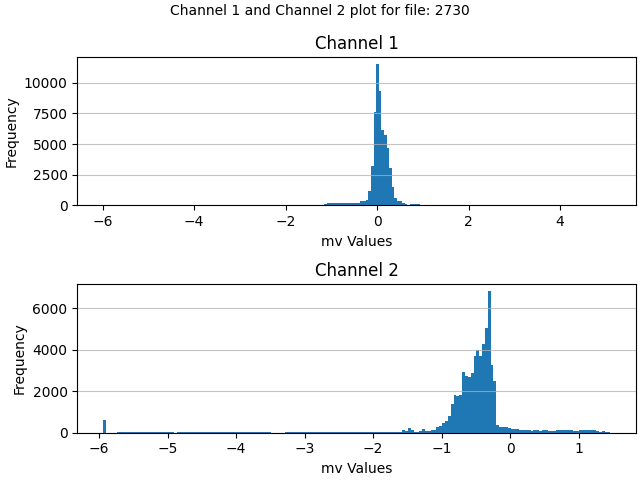
\includegraphics[width=1.0\linewidth, height=8cm]{BachelorMasterThesis/DataExploration/Figures/atrial_fibrillation/histogram/2730.png}
%             % \captionof{figure}{Mathematical model of the neuron 4}
%             \label{fig:af_histogram_4}
%     \end{minipage}
%     \caption{ECG signal distribution - Histogram - of Sinus (left) vs Atrial fibrillation (right)}
%     \label{fig:ecg_histogram_plot_2_sinus_vs_af}
% \end{figure}

\begin{figure}[ht!]
\centering
    \begin{minipage}{.5\textwidth}
      \centering
        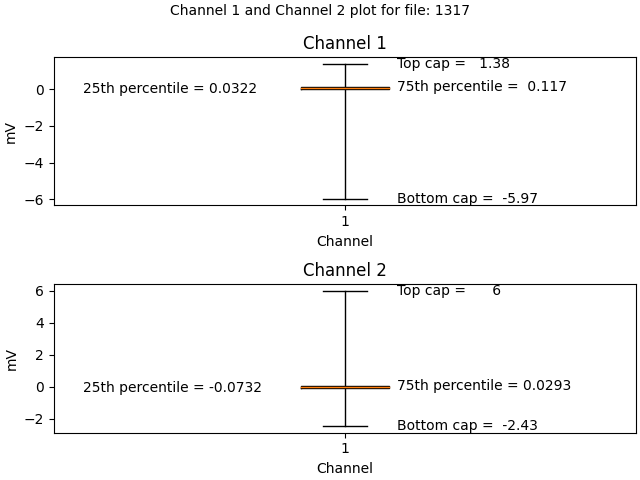
\includegraphics[width=1.0\linewidth, height=8cm]{BachelorMasterThesis/DataExploration/Figures/sinus/box_plot/1317_box.png}
            % \captionof{figure}{Mathematical model of the neuron 3}
            \label{fig:sinus_box_1}
        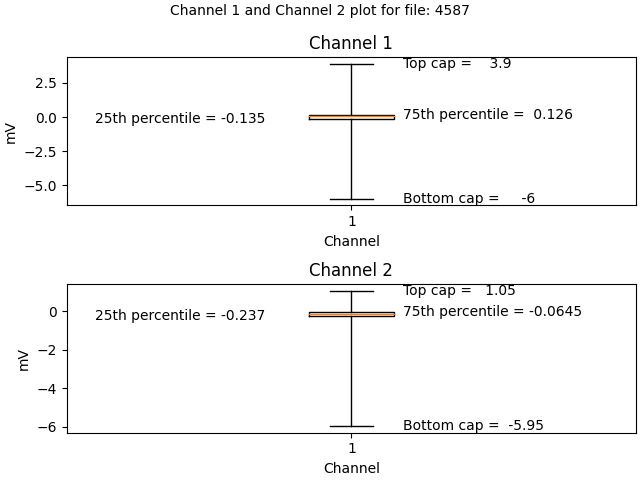
\includegraphics[width=1.0\linewidth, height=8cm]{BachelorMasterThesis/DataExploration/Figures/sinus/box_plot/4587_box.png}
            % \captionof{figure}{Mathematical model of the neuron 2}
            \label{fig:sinus_box_2}
    \end{minipage}%
    \begin{minipage}{.5\textwidth}
      \centering
        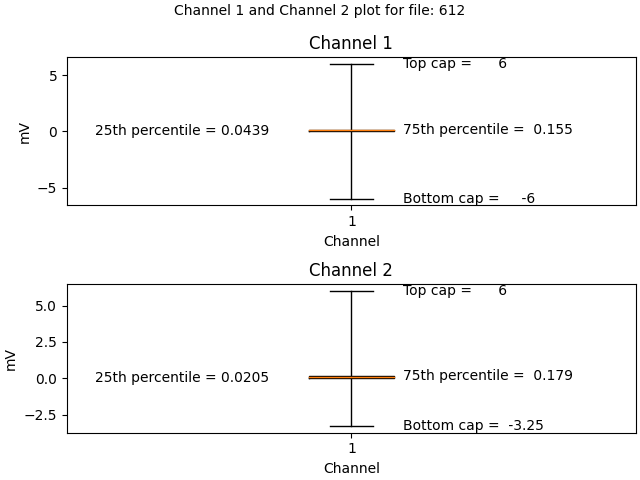
\includegraphics[width=1.0\linewidth, height=8cm]{BachelorMasterThesis/DataExploration/Figures/atrial_fibrillation/box_plot/612_box.png}
            % \captionof{figure}{Biological Neuron 1}
            \label{fig:af_box_1}
        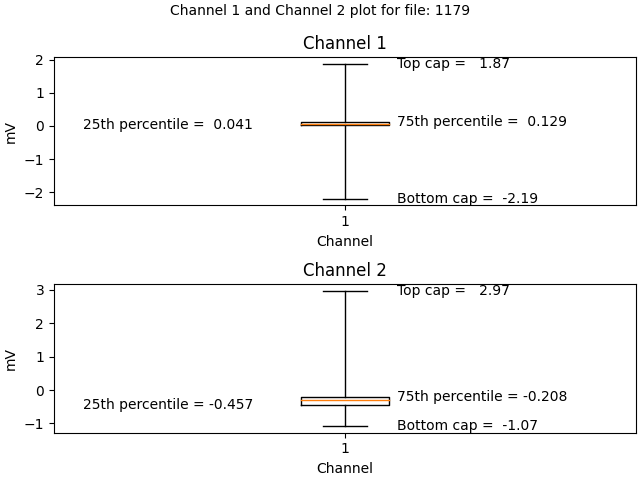
\includegraphics[width=1.0\linewidth, height=8cm]{BachelorMasterThesis/DataExploration/Figures/atrial_fibrillation/box_plot/1179_box.png}
            % \captionof{figure}{Mathematical model of the neuron 3}
            \label{fig:af_box_2}
    \end{minipage}
    \caption{ECG signal distribution - box plot - of Sinus (left) vs Atrial fibrillation (right)}
    \label{fig:ecg_box_plot_1_sinus_vs_af}
\end{figure}

% \begin{figure}[ht!]
% \centering
%     \begin{minipage}{.5\textwidth}
%       \centering
%         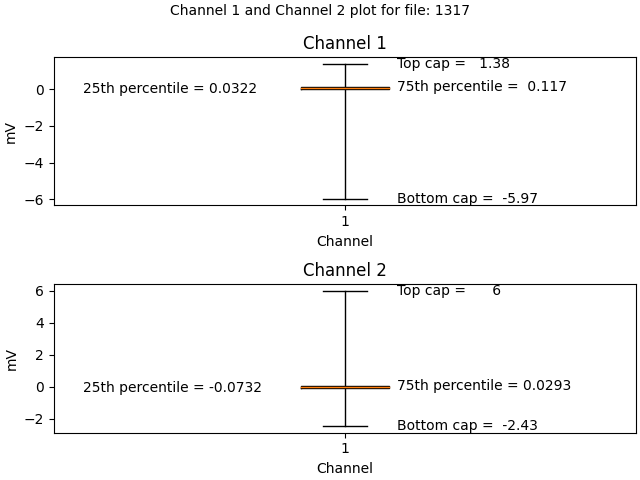
\includegraphics[width=1.0\linewidth, height=8cm]{BachelorMasterThesis/DataExploration/Figures/sinus/box_plot/1317_box.png}
%             % \captionof{figure}{Biological Neuron 1}
%             \label{fig:sinus_box_3}
%         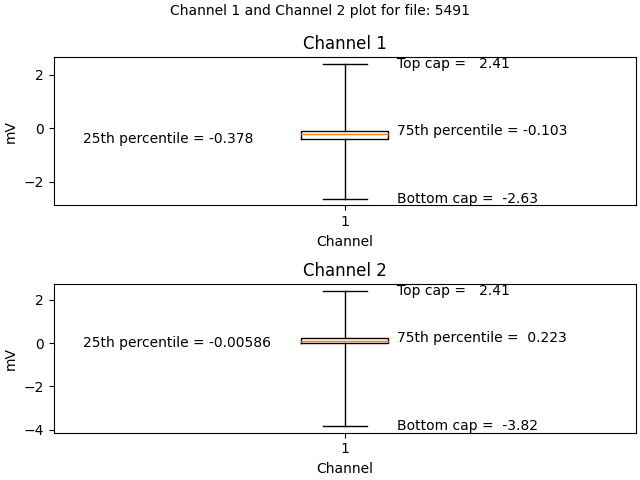
\includegraphics[width=1.0\linewidth, height=8cm]{BachelorMasterThesis/DataExploration/Figures/sinus/box_plot/5491_box.png}
%             % \captionof{figure}{Mathematical model of the neuron 4}
%             \label{fig:sinus_box_4}
%     \end{minipage}%
%     \begin{minipage}{.5\textwidth}
%       \centering
%         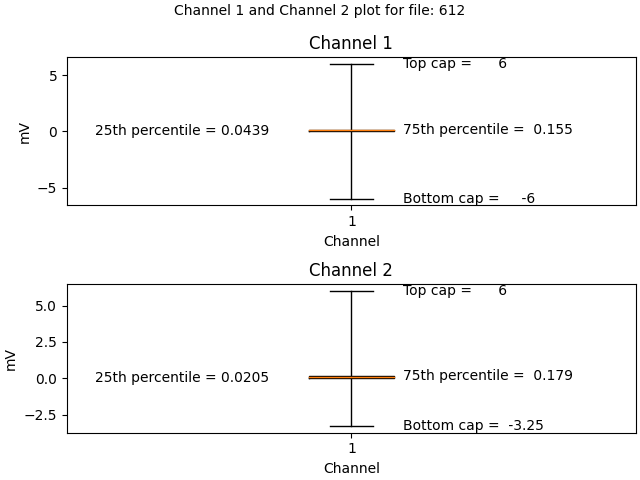
\includegraphics[width=1.0\linewidth, height=8cm]{BachelorMasterThesis/DataExploration/Figures/atrial_fibrillation/box_plot/612_box.png}
%             % \captionof{figure}{Mathematical model of the neuron 2}
%             \label{fig:af_box_3}
%         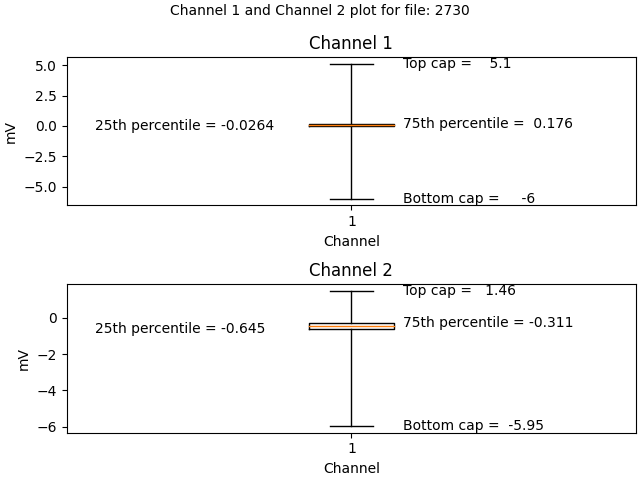
\includegraphics[width=1.0\linewidth, height=8cm]{BachelorMasterThesis/DataExploration/Figures/atrial_fibrillation/box_plot/2730_box.png}
%             % \captionof{figure}{Mathematical model of the neuron 4}
%             \label{fig:af_box_4}
%     \end{minipage}
%     \caption{ECG signal distribution - box plot - of Sinus (left) vs Atrial fibrillation (right)}
%     \label{fig:ecg_box_plot_2_sinus_vs_af}
% \end{figure}

\clearpage

\section{Data analysis}
\label{sec:data_analysis}

When a normal ECG signal is provided, the detection of atrial fibrillation within the ECG signal is problematic as it may be episodic. Figure~\ref{fig:ecg_sinus_vs_af} shows the ECG signal of the sinus rhythm (left) and atrial fibrillation (right). There were 4 files chosen randomly from both sinus and atrial fibrillation and the voltage values obtained for two channels were plotted. The $y-axis$ represent the voltage values (in mV) and $x-axis$ represents time (in seconds). As seen from these graphs, it is hard to distinguish an atrial fibrillation signal from a normal sinus rhythm signal just by observing them.

Next, we focus on the frequency distribution of the data for the same 4 ECG files from sinus and atrial fibrillation using histograms \cite{scott1979optimal}. The data is unfiltered and not prepossessed. The histogram for the 2 channels for these files are shown in Figure~\ref{fig:ecg_histogram_plot_1_sinus_vs_af}. As seen from most of these histogram plots, the voltage values are concentrated around zero (between -1mV and 1mV) with occasional values exceeding -1mV or 1mV. Although most of the values are concentrated around zero, those zero values are because of the cardiac cycle and not because of the disconnection or disturbance in transmission. The occasional values exceeding -1mV or 1mV are the spikes seen in the ECG graph (Figure~\ref{fig:ecg_sinus_vs_af}). 

Again, it is not very easy to distinguish between an atrial fibrillation signal and a sinus signal from these histogram plots. For example, the histogram of channel 1 and channel 2 values for sinus file 1317 and atrial fibrillation file 612 are very similar. This is the general observation throughout the dataset. Also, it is not easy to determine outliers from histograms.

Further, to understand and compare the distribution of the data points, we create box and whisker plots for the same 4 ECG files of sinus and atrial fibrillation (Figure~\ref{fig:ecg_box_plot_1_sinus_vs_af}). A box and whisker plot is a visual representation that provides information about the minimum value, first quartile, median (second quartile), third quartile, and maximum of a set of values. The box and whisker plots can provide information about outliers, the data symmetry and how tightly the data is grouped. It also provides information on the variability or dispersion of the data \cite{mcgill1978variations} \& \cite{krzywinski2014points}. 

As seen from Figure~\ref{fig:ecg_box_plot_1_sinus_vs_af}, 
The majority of the voltage values are in between -1mV and 1mV. We also note that there are not outliers in the distribution. This signifies that the ECG data in the dataset is clean enough to try to proceed in building the machine learning model for this dataset without significant prepossessing. We speak about the architecture, experiments, and results in the next section.

\section{Seed Model}
\label{sec:seed_model}

With this analysis of data, we wanted to proceed and check if CNN models are sufficient to classify the dataset. The goal is to design one or more CNN models which can be used as seed models to achieve the training and validation accuracy of greater than 90\% for the training and validation dataset. Also, the authors from the paper \cite{real2019regularized} mention that starting with a high-quality model in the initial stages while using neural architecture search increases the probability to get a higher quality model in the end.

For the training process, the standard TensorFlow input pipeline is used. From the 11,200 files (5,600 for sinus rhythm and 5,600 for atrial fibrillation), we create a TFRecord file for training. A TFRecord is created to serialize the data and to read it back efficiently and linearly. With 2 channel data for a single ".ecg" file, in this work, we limit the number of samples per channel to be 60,000 (which is precisely the data for 2 minutes). We prevent the rest of the samples from being written to the TFRecord. With this, we essentially create a binary record of the 11,200 files. Similarly, TFRecords for testing and validation each with 2,400 files (1,200 for sinus rhythm and 1,200 for atrial fibrillation) are created.

TFRecord dataset APIs of TensorFlow are used to read the data from the TFRecords. The dataset API also helps to shuffle the TFRecord data as this also becomes critical to randomly distribute the data. After developing this pipeline, the architectures in Figure~\ref{fig:seed_model_1_n_2} are used to train the two seed models.

\begin{figure}[ht!]
\centering
    \begin{tabular}{@{}c@{}}
        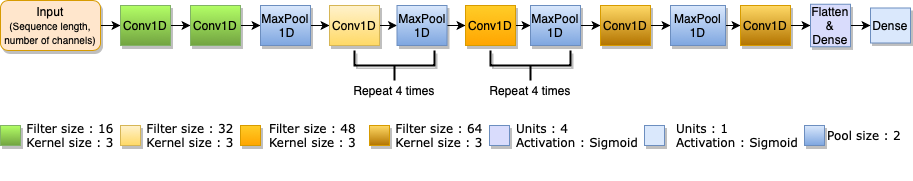
\includegraphics[width=1.0\linewidth, height=5cm]{BachelorMasterThesis/DataExploration/Figures/Seed_model_2.png}  \\[\abovecaptionskip]
            % \captionof{seed_model_2_architecture}{Seed model 2 architecture}
        % \label{fig:seed_model_2_architecture}
        \small (a) Seed model with additional convolutional and dense layers
    \end{tabular}
    
     \vspace{\floatsep}
    
    \begin{tabular}{@{}c@{}}
        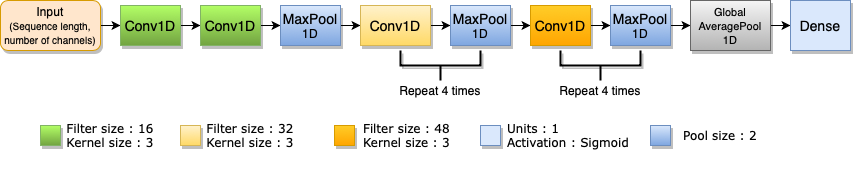
\includegraphics[width=1.0\linewidth, height=5cm]{BachelorMasterThesis/DataExploration/Figures/Seed_model.png}  \\[\abovecaptionskip]
            % \captionof{seed_model_architecture}{Seed model architecture}
        % \label{fig:seed_model_architecture}
        \small (b) Seed model with Global average pooling
    \end{tabular}
    \caption{Seed Models}
    \label{fig:seed_model_1_n_2}
\end{figure}

The first seed model in Figure~\ref{fig:seed_model_1_n_2} (a) is developed to use CNN layers to classify the dataset with the minimum number of parameters as possible. After developing this model, we tried to explore the possibility of further reducing the complexity of the model. The thought process was to avoid the use of fully connected layers (dense layers) for the model. This was accomplished by using a 1-dimensional global average pool layer which not only flattens the input from the previous layer, but also reduces the number parameters of the entire model (Figure~\ref{fig:seed_model_1_n_2} (b)). This results in reduced complexity with the same hyperparameter settings.

The architectures in Figure~\ref{fig:seed_model_1_n_2} (a) and (b) consists of a 1-dimensional TensorFlow input layer. This layer takes the sequence length (fixed at $60000$) and the number of channels ($2$ channels provided in the dataset) as the input. This is followed by two 1-dimensional convolutional layers, each having a filter size and kernel size of $16$ and $3$ respectively. These convolutional layers are followed by a 1-dimensional max pool layer (with pool size $2$ to half the first dimension of the data). The max pool layer is followed by a set of convolutional layer (filter size of $32$ and kernel size of $3$) and a max pool layer (with pool size $2$), repeated 4 times in that order. This is followed by another set of convolutional layer (filter size of $48$ and kernel size of $3$) and a max pool layer (with pool size $2$), repeated 4 times in that order. The architecture structure is similar for both seed models up to this point.

For the architecture in Figure~\ref{fig:seed_model_1_n_2} (a), the max pool layer is followed by a 1-dimensional convolutional layer (filter size of $64$ and kernel size $3$), a max pool layer (with pool size $2$) and another convolutional layer (filter size of $64$ and kernel size $3$). These layers are followed by a flattening layer which flattens the data for the dense layer (fully connected layer), which uses 4 neurons. In the end, a dense layer with a single neuron for classification is used.

For the architecture in Figure~\ref{fig:seed_model_1_n_2} (b), the max pool layer is followed by a 1-dimensional global average pool layer which flattens the data for the dense layer which is used for classification.

All the convolutional layers use "\textbf{ReLU}" activation, whereas the dense layer uses a sigmoid activation. The sigmoid activation is used to classify the result either to '$0$' (sinus rhythm) or '$1$' (atrial fibrillation). For both models the "\textbf{Adam}" optimizer is used with a learning rate of \textbf{$4e^{-4}$} and decay rate of \textbf{$1e^{-3}$}. As we are performing binary classification, binary cross-entropy is used as a loss function. The TFRecord for validation is passed for performing validation for the training process. The accuracy metric along a batch size of $32$ is used for both training and validation. With these conditions, we train the models for $5$ epochs. The models are then tested for the test data (TFRecord for test data). The models result in very good testing accuracy, thus confirming our intuition that CNN models are sufficient to classify this dataset. The results for the seed models are mentioned in \autoref{sec:seed_model_experiments}.

\subsubsection{Hyperparameters}
\label{sec:hyperparameters}

The hyperparameters used for the seed models are described in Table~\ref{table:hyperparameters}. These hyperparameters are derived by experimenting with the seed models. They set the foundation for the NAS, as the same set of hyperparameters are also used for the NAS process.

\begingroup
\setlength{\tabcolsep}{10pt}
\renewcommand{\arraystretch}{1.5}
\begin{table}[ht]
\centering
\begin{tabular}{|c|c|}
\hline
{\textbf{Hyperparameter}}  & { \textbf{Value}} \\ \hline

Optimizer           & Adam          \\ \hline
Learning rate       & $4e^{-4}$     \\ \hline
Decay               & $1e^{-3}$     \\ \hline
Number of epochs    & 5             \\ \hline
Batch size          & 32            \\ \hline
Max runtime seconds & 300 s         \\ \hline
Training Samples    & 11200         \\ \hline
Validation Samples  & 2400          \\ \hline
Testing Samples     & 2400          \\ \hline
\begin{tabular}[c]{@{}c@{}}Steps per epoch \\ (training samples / batchsize)\end{tabular} & 350                                   \\ \hline
\begin{tabular}[c]{@{}c@{}}Validation steps\\ (validation steps / batchsize)\end{tabular} & 75                                    \\ \hline
\end{tabular}
\caption{Hyperparameters used for the seed models}
\label{table:hyperparameters}
\end{table}
\endgroup